\documentclass[../Article_Model_Parameters.tex]{subfiles}
\graphicspath{{\subfix{../Figures/}}}
\begin{document}
	
	\label{CH: Results}
	
	Some results of the parameter estimations

	\begin{figure*}
		\centering
		\begin{subfigure}[b]{0.7\textwidth}
			\centering
			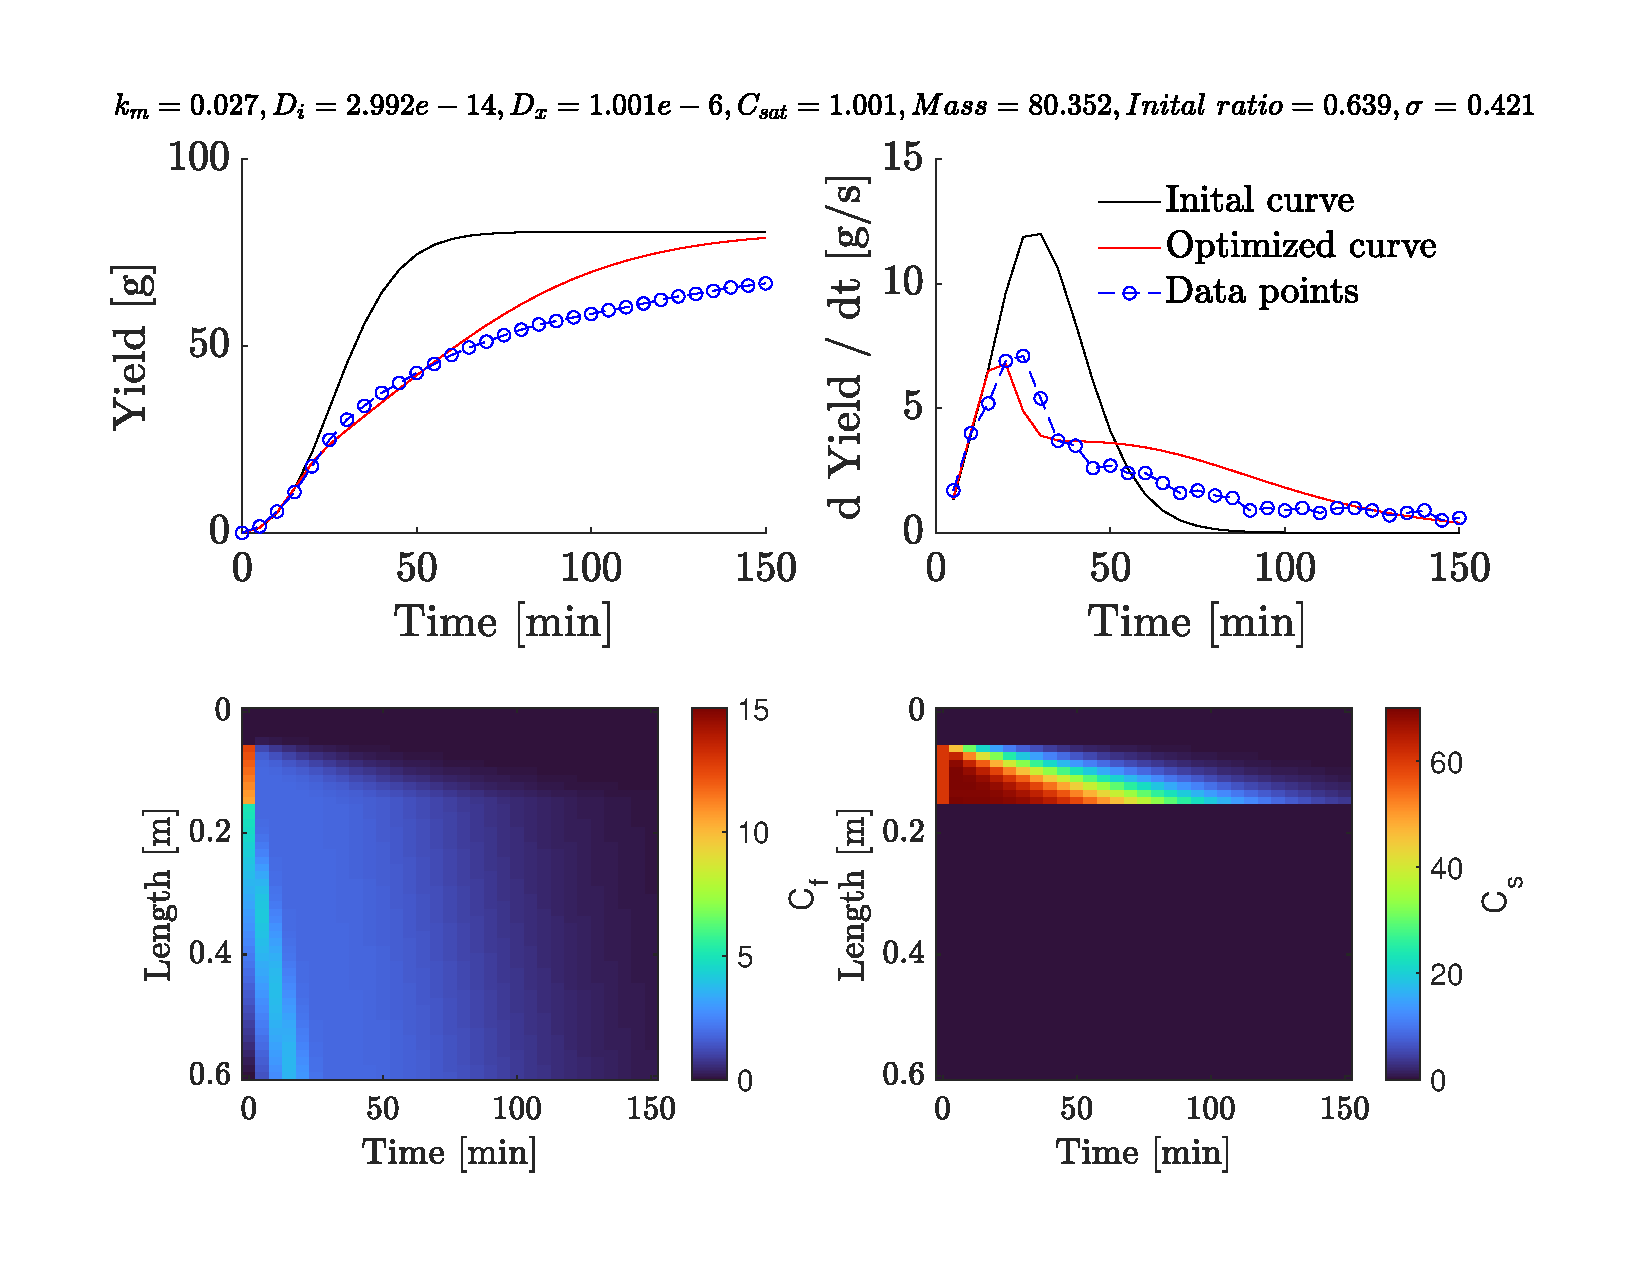
\includegraphics[trim = 3cm 11cm 2.5cm 1cm,clip,width=\textwidth]{/Results_estimation/Fitting_LUKE_T40_P200.pdf}
			\caption{Experiment at $40^\circ C$ and $200$ bar}
		\end{subfigure}
		\hfill
		\begin{subfigure}[b]{0.7\textwidth}
			\centering
			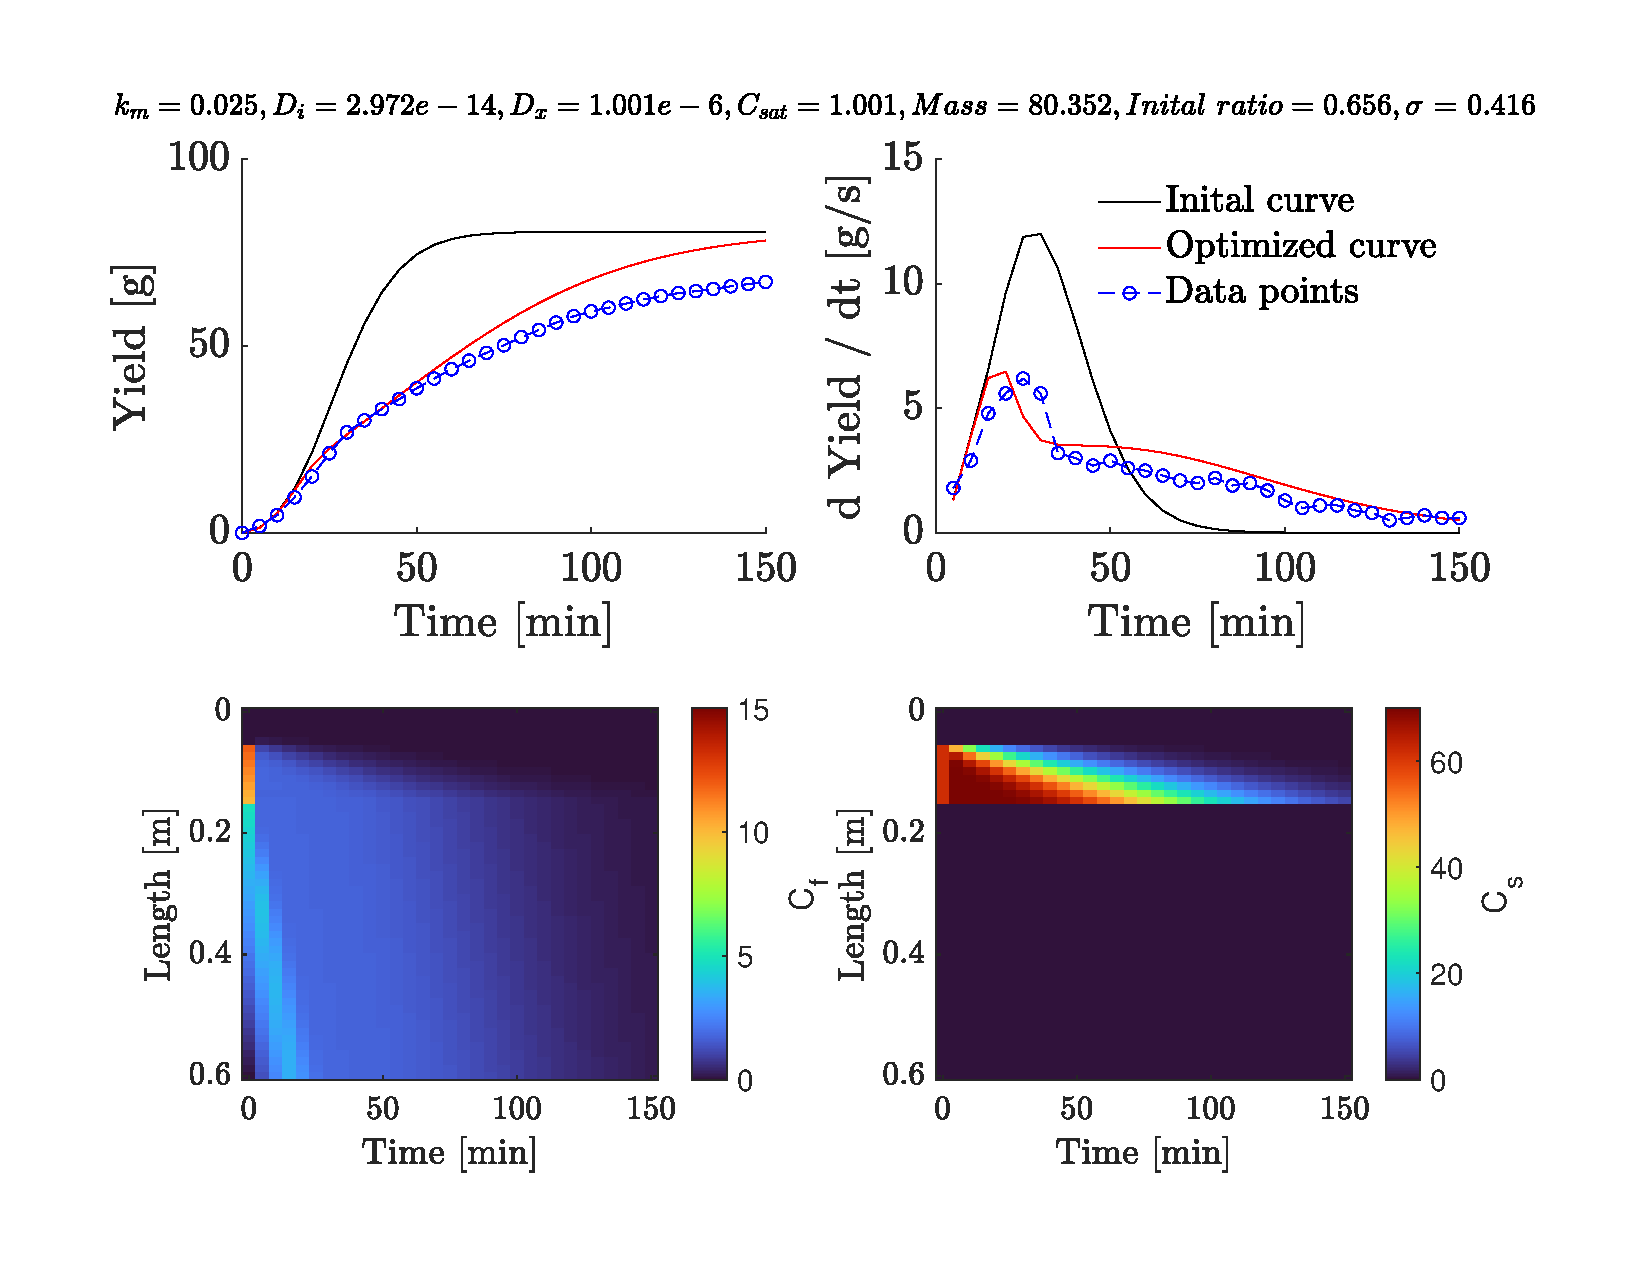
\includegraphics[trim = 3cm 11cm 2.5cm 1cm,clip,width=\textwidth]{/Results_estimation/Fitting_LUKE_T50_P200.pdf}
			\caption{Experiment at $50^\circ C$ and $200$ bar}
		\end{subfigure}
		\hfill
		\begin{subfigure}[b]{0.7\textwidth}
			\centering
			\includegraphics[trim = 3cm 11cm 2.5cm 1cm,clip,width=\textwidth]{/Results_estimation/Fitting_LUKE_T40_P300_org.pdf}
			\caption{Experiment at $40^\circ C$ and $300$ bar}
		\end{subfigure}
		\hfill
		\begin{subfigure}[b]{0.7\textwidth}
			\centering
			\includegraphics[trim = 3cm 11cm 2.5cm 1cm,clip,width=\textwidth]{/Results_estimation/Fitting_LUKE_T50_P300_org.pdf}
			\caption{Experiment at $50^\circ C$ and $300$ bar}
		\end{subfigure}
		\caption{Results of parameter fitting, with estimation of the initial state}
	\end{figure*}

	\begin{figure*}
	\centering
	\begin{subfigure}[b]{0.85\textwidth}
		\centering
		\includegraphics[trim = 1cm 2cm 2.5cm 1cm,clip,width=\textwidth]{/Results_estimation/Trend_Lines_order_1.pdf}
		\caption{First order polynomial regression of fitted parameters as a function of fluid density $\rho_f$}
	\end{subfigure}
	\hfill
	\begin{subfigure}[b]{0.85\textwidth}
		\centering
		\includegraphics[trim = 1cm 2cm 2.5cm 1cm,clip,width=\textwidth]{/Results_estimation/Trend_Lines_order_2.pdf}
		\caption{Second order polynomial regression of fitted parameters as a function of fluid density $\rho_f$}
	\end{subfigure}
	\caption{Results of parameter fitting, with estimation of the initial state}
\end{figure*}
		
	
\end{document}